\documentclass[12pt,a4paper]{article}

% Пакеты для кодировки и шрифтов
\usepackage{fontspec}
\usepackage{polyglossia}
\setmainlanguage{russian}
\setotherlanguage{english}

\setmainfont{Liberation Serif} % Альтернативы: Times New Roman, DejaVu Serif
\setmonofont{DejaVu Sans Mono}  % Для программирования
% Математические пакеты
\usepackage{amsmath}
\usepackage{amsfonts}
\usepackage{amssymb}
\usepackage{listings}

% Для работы с графикой
\usepackage{graphicx}
\usepackage{float}

% Для красивого оформления
\usepackage{xcolor}
\usepackage{hyperref}
\usepackage{geometry}
\geometry{left=2.5cm,right=2.5cm,top=2cm,bottom=2cm}

\lstset{
    basicstyle=\ttfamily\small,
    keywordstyle=\color{blue},
    commentstyle=\color{green!50!black},
    stringstyle=\color{red},
    numbers=left,
    numberstyle=\tiny\color{gray},
    stepnumber=1,
    numbersep=5pt,
    backgroundcolor=\color{gray!5},
    frame=single,
    rulecolor=\color{gray},
    breaklines=true,
    captionpos=b,
    tabsize=4,
    showspaces=false,
    showstringspaces=false
}

\lstdefinestyle{python}{
    language=Python,
    morekeywords={as, async, await, None, True, False}
}

% Настройка гиперссылок
\hypersetup{
    colorlinks=true,
    linkcolor=blue,
    urlcolor=red,
    pdftitle={report}
}

\begin{document}

% Основное содержимое
\section{Установка зависимостей}

В первой клетке документа мы установили зависимости в виртуальное окружение. Для этого был написан файл requirements.txt следующего содержания:

\begin{lstlisting}
# ============================================
# PyTorch + ROCm (AMD GPU support)
# ============================================
torch==2.4.1+rocm6.1
torchvision==0.19.1+rocm6.1
torchaudio==2.4.1+rocm6.1
--extra-index-url https://download.pytorch.org/whl/rocm6.1

# ============================================
# Core ML / Data Science Libraries
# ============================================
numpy
pandas
scipy
scikit-learn
matplotlib
seaborn
opencv-python
Pillow
tqdm

# ============================================
# Jupyter environment
# ============================================
jupyterlab
notebook

# ============================================
# Deep Learning Tools / Model Deployment
# ============================================
onnx
onnxruntime-gpu
albumentations
\end{lstlisting}

\section{GPU-отчёт}

Далее, была выведена модель CUDA-устройства и количество VRAM.
\begin{lstlisting}
 Device Name           | Total Memory (GB)
-----------------------|-------------------
 AMD Radeon RX 6600    | 7.98
\end{lstlisting}

Данная лабораторная работа выполнялась на AMD Radeon RX 6600 с 8 гигабайтами VRAM. Для имитации CUDA использовался бекенд ROCm.

\section{Альбументо-аугментации}

В качестве базы была взята готовая модель EfficientNet-B3. Для улучшения качества модели была использована библиотека albumentations. Итоговая точность дообученной модели составила 92.42\%. График представлен на рис. 1.

\begin{figure}[ht]
    \centering
    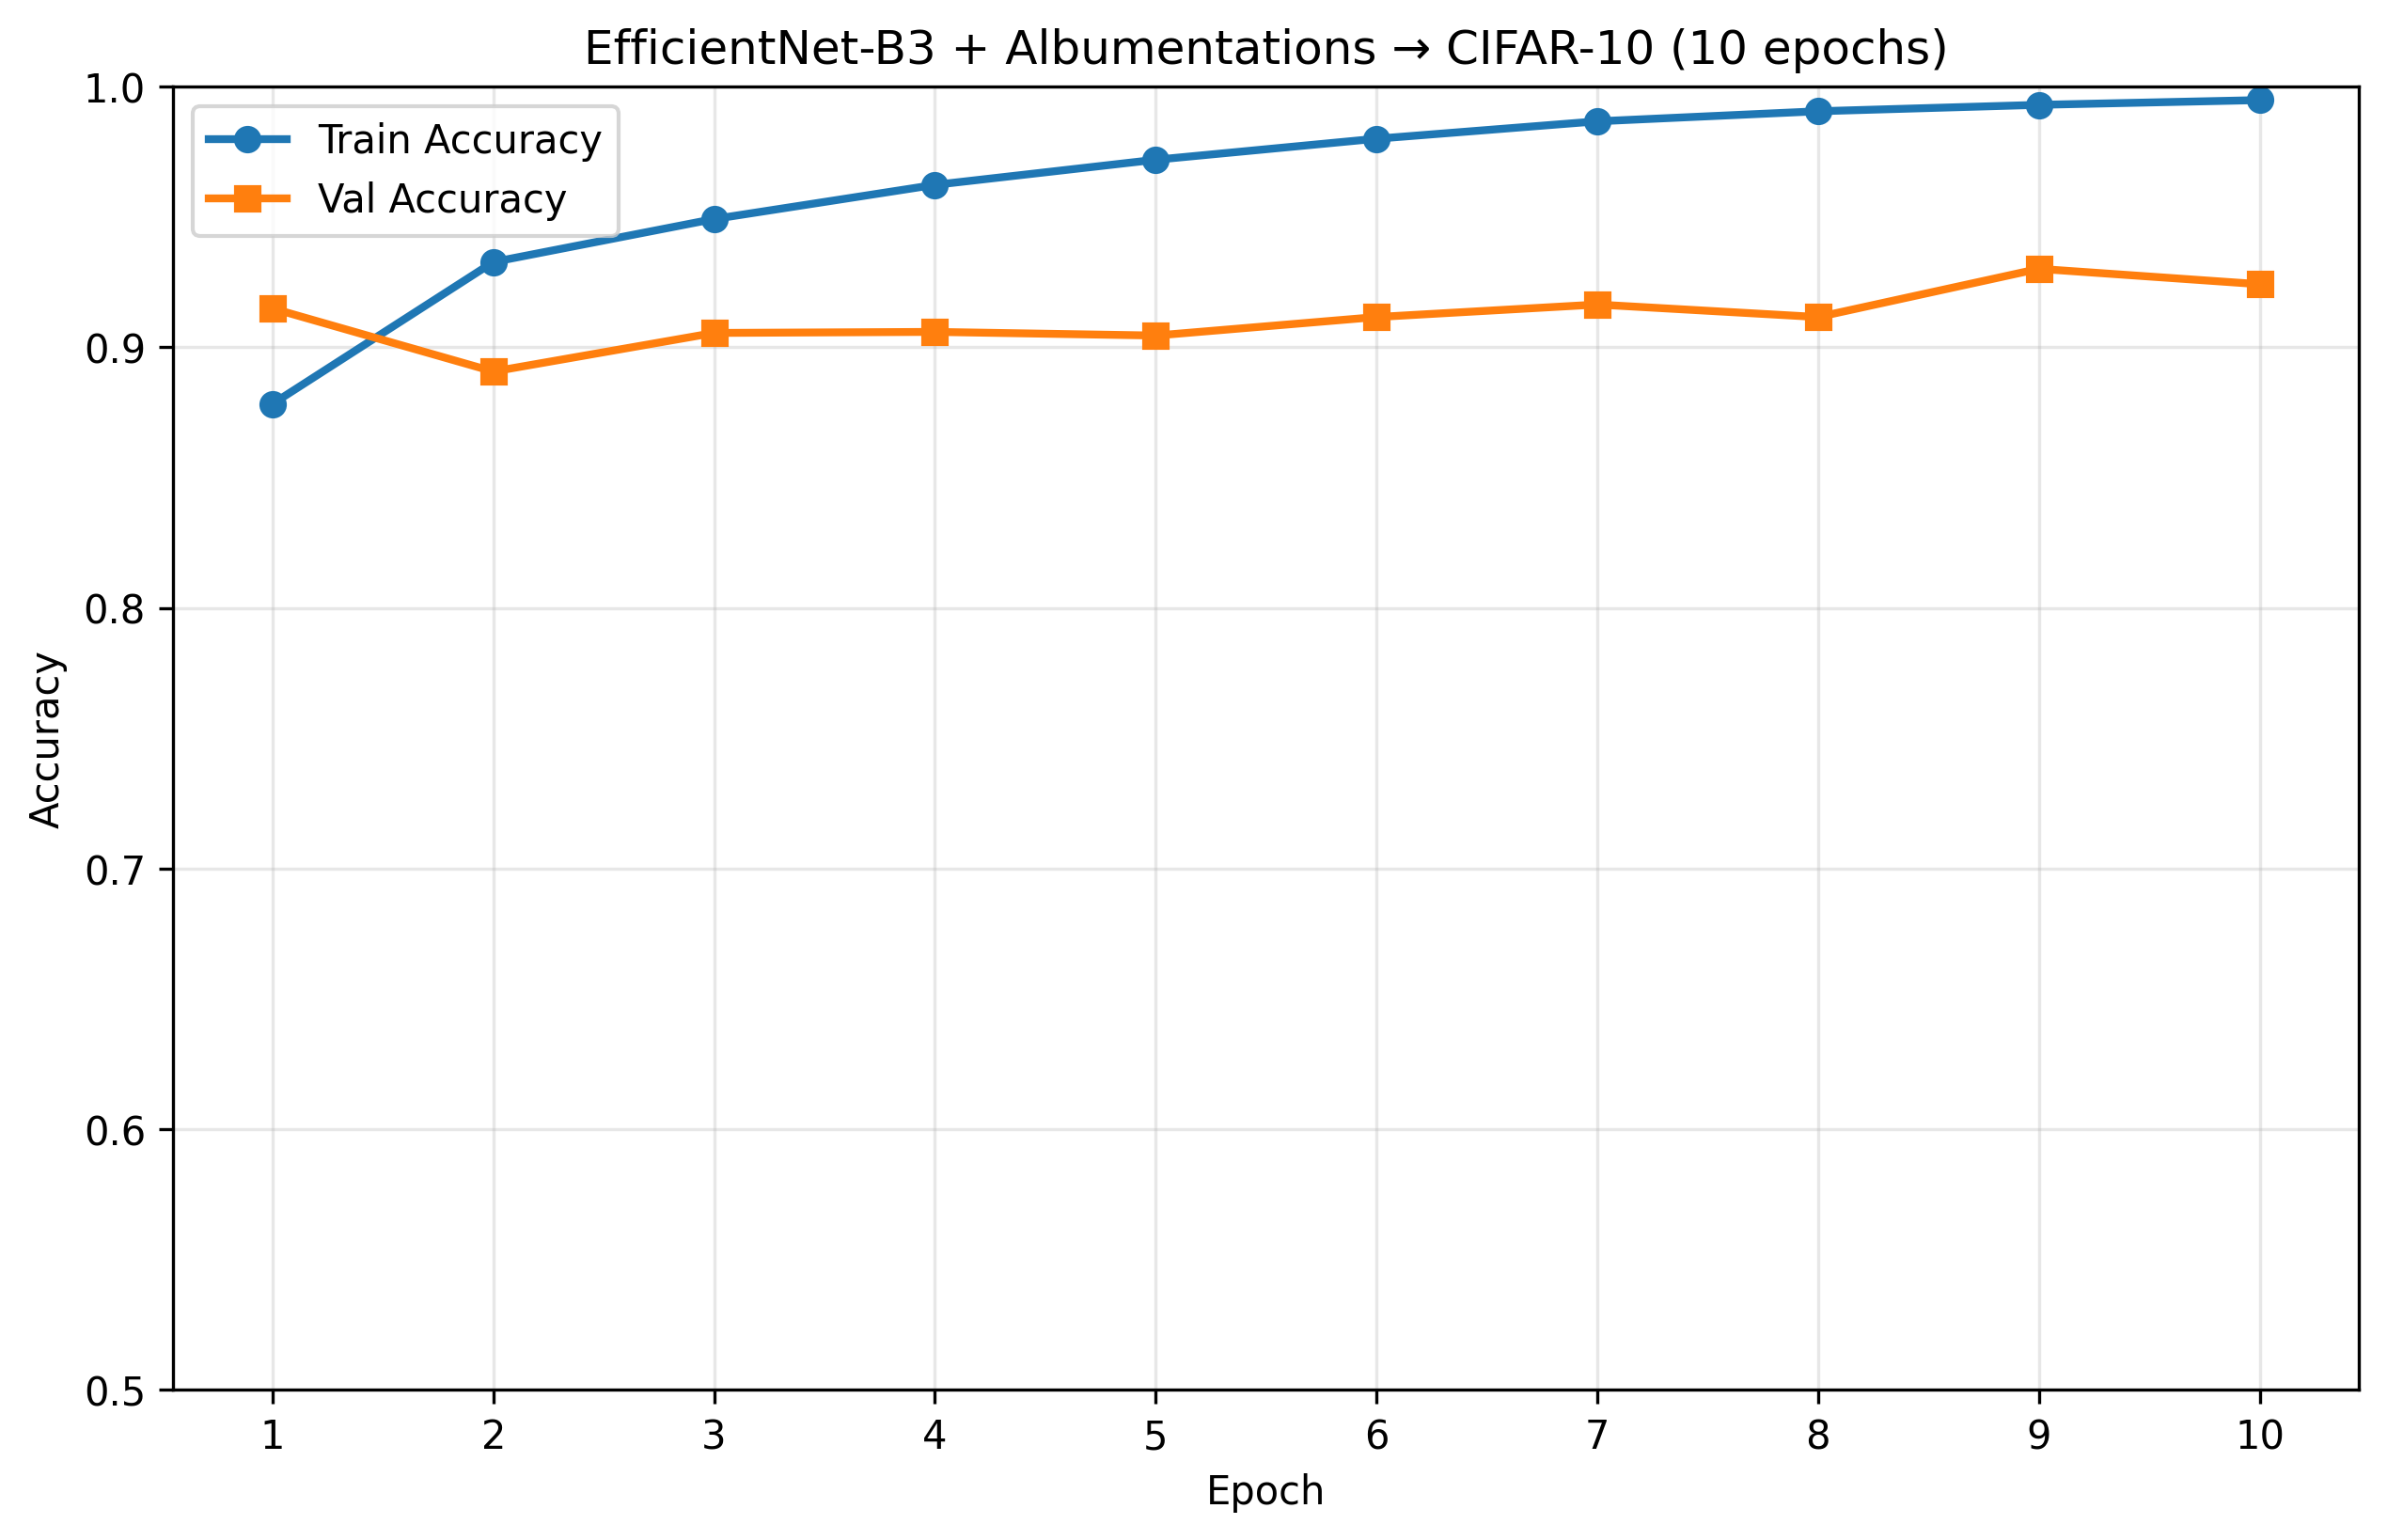
\includegraphics[width=0.8\textwidth]{docs/accuracy_plot_b3.png}
    \caption{График точности дообученной EfficientNet-B3}
    \label{fig:accuracy_plot}
\end{figure}

\section{A/B EfficientNet}

Далее тот же процесс был проделан на EfficientNet-B0. Итоговая точность составила 92.85\%. График представлен на рис. 2.

\begin{figure}[ht]
    \centering
    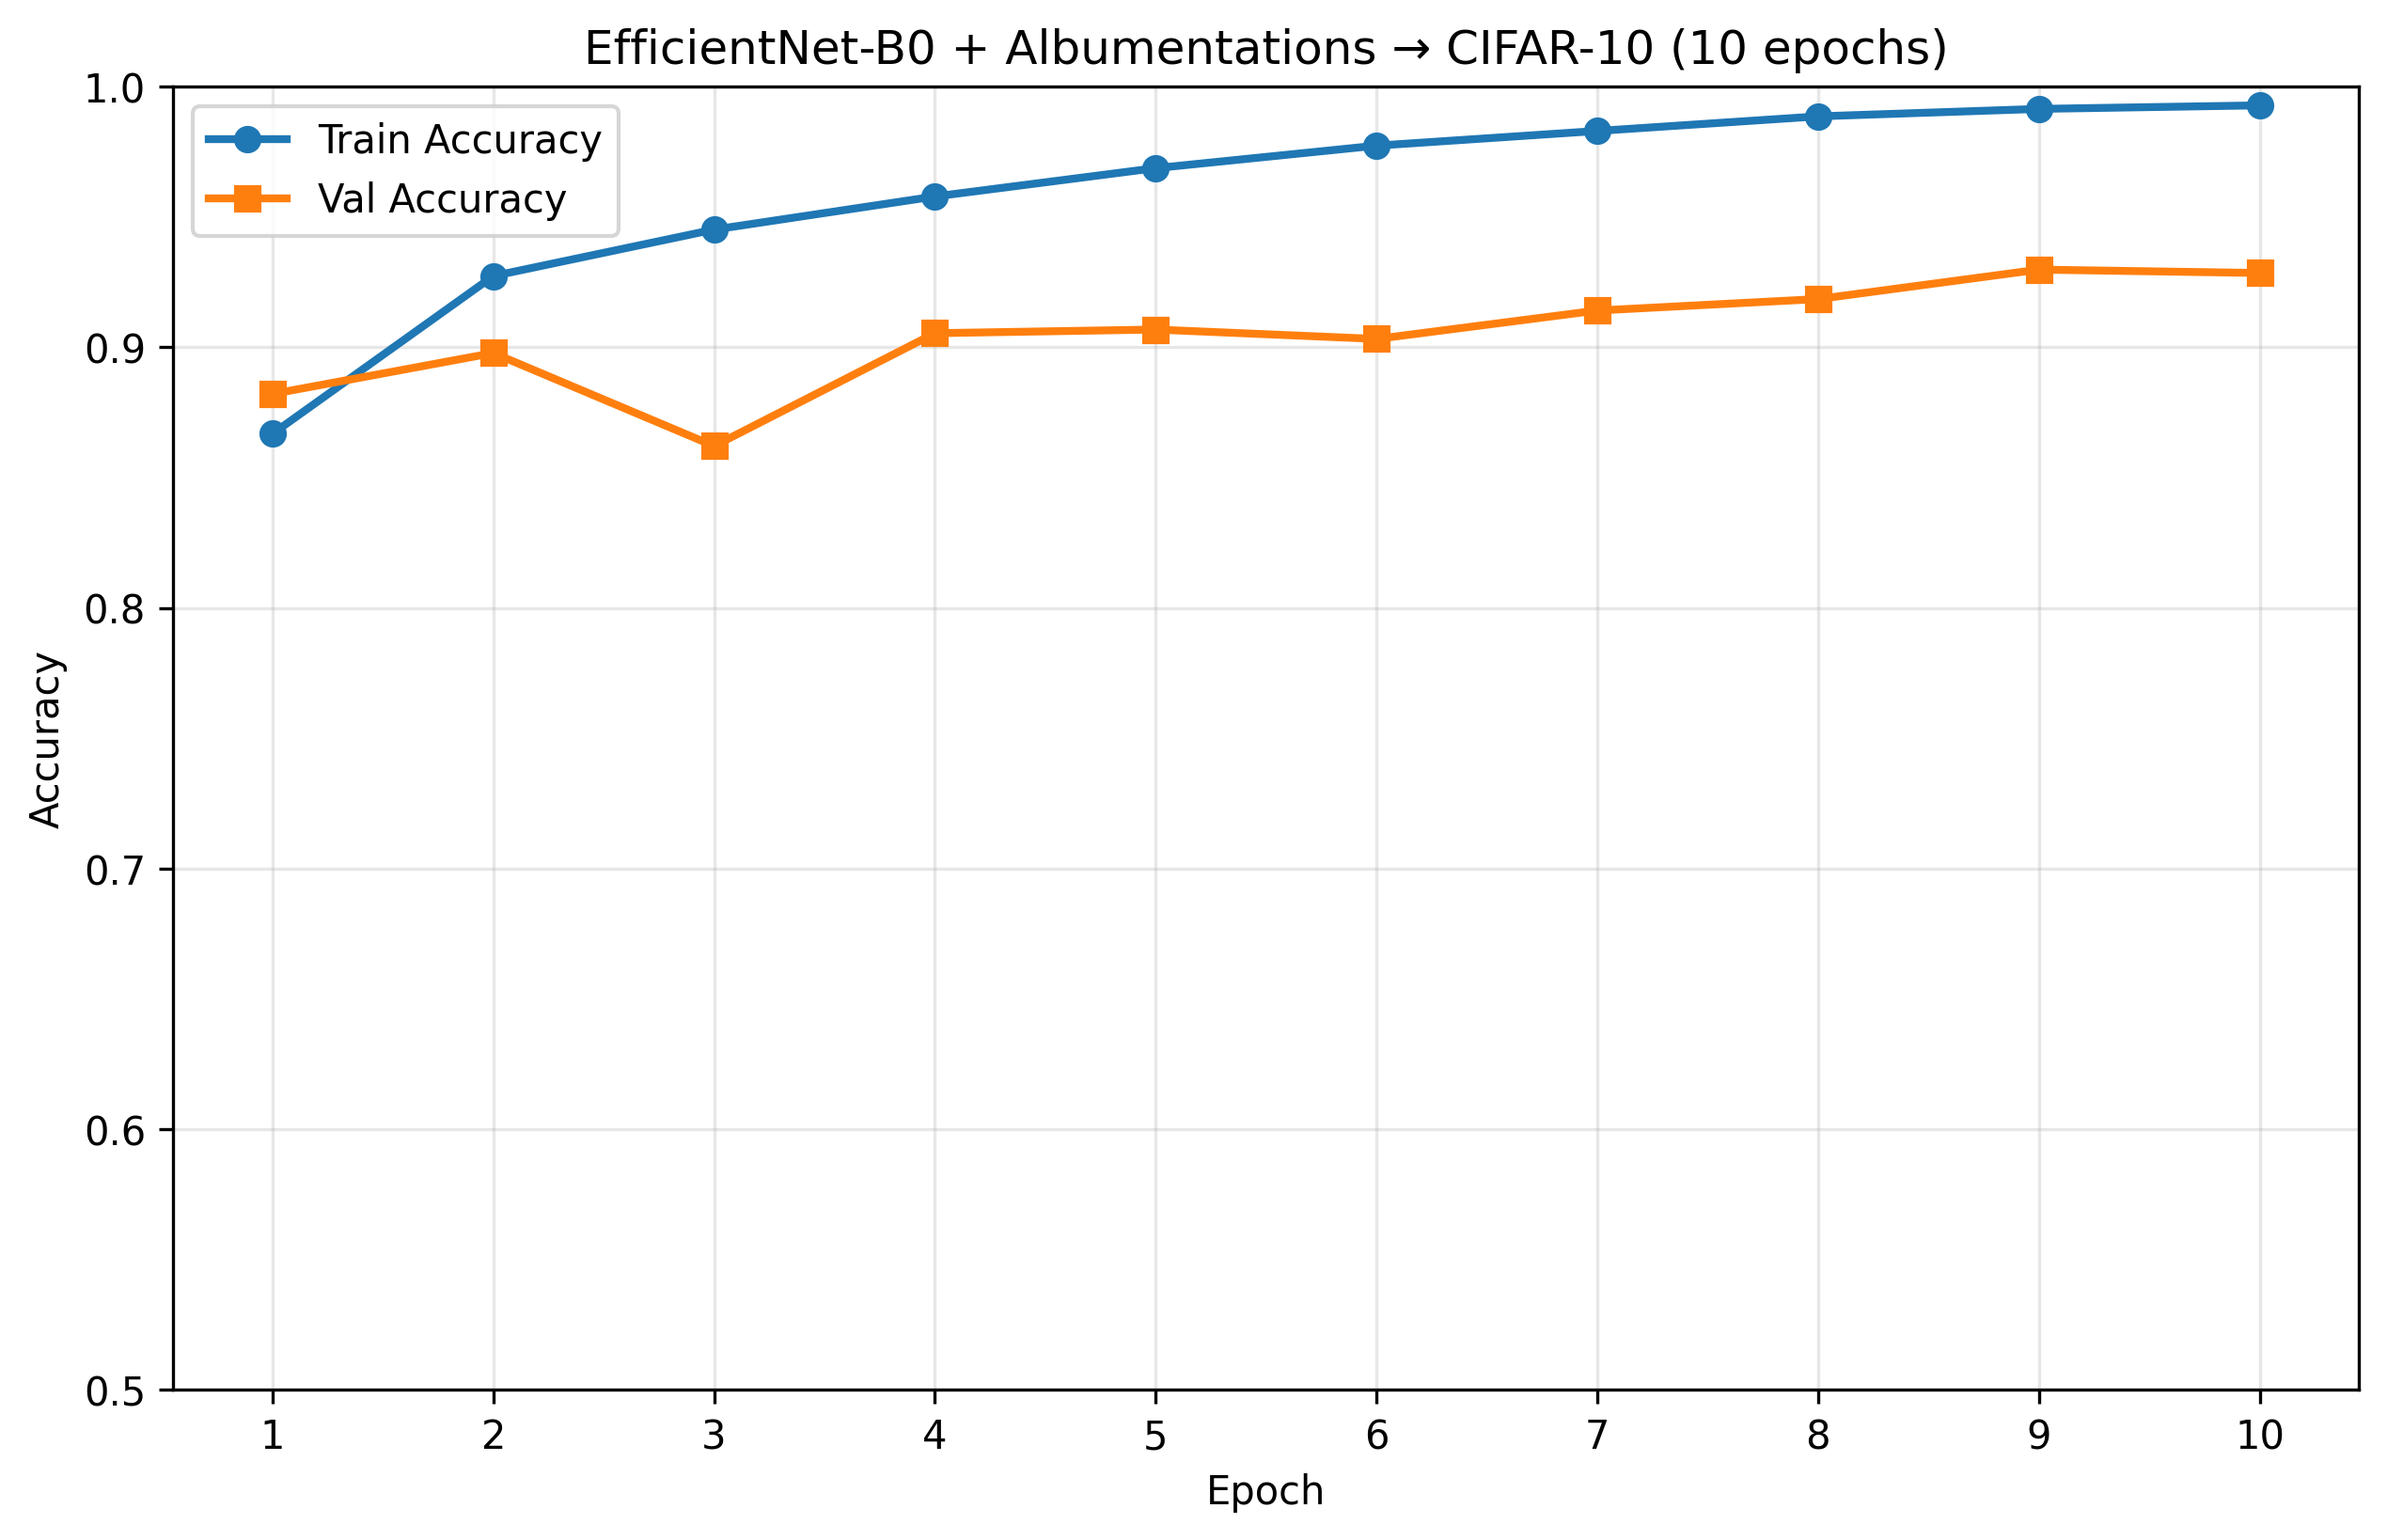
\includegraphics[width=0.8\textwidth]{docs/accuracy_plot_b0.png}
    \caption{График точности дообученной EfficientNet-B0}
    \label{fig:accuracy_plot}
\end{figure}

\section{Early Stopping}

Была добавлена клетка с ранней остановкой обучения в случае, если валидационная точность перестаёт улучшаться.

\begin{figure}[ht]
    \centering
    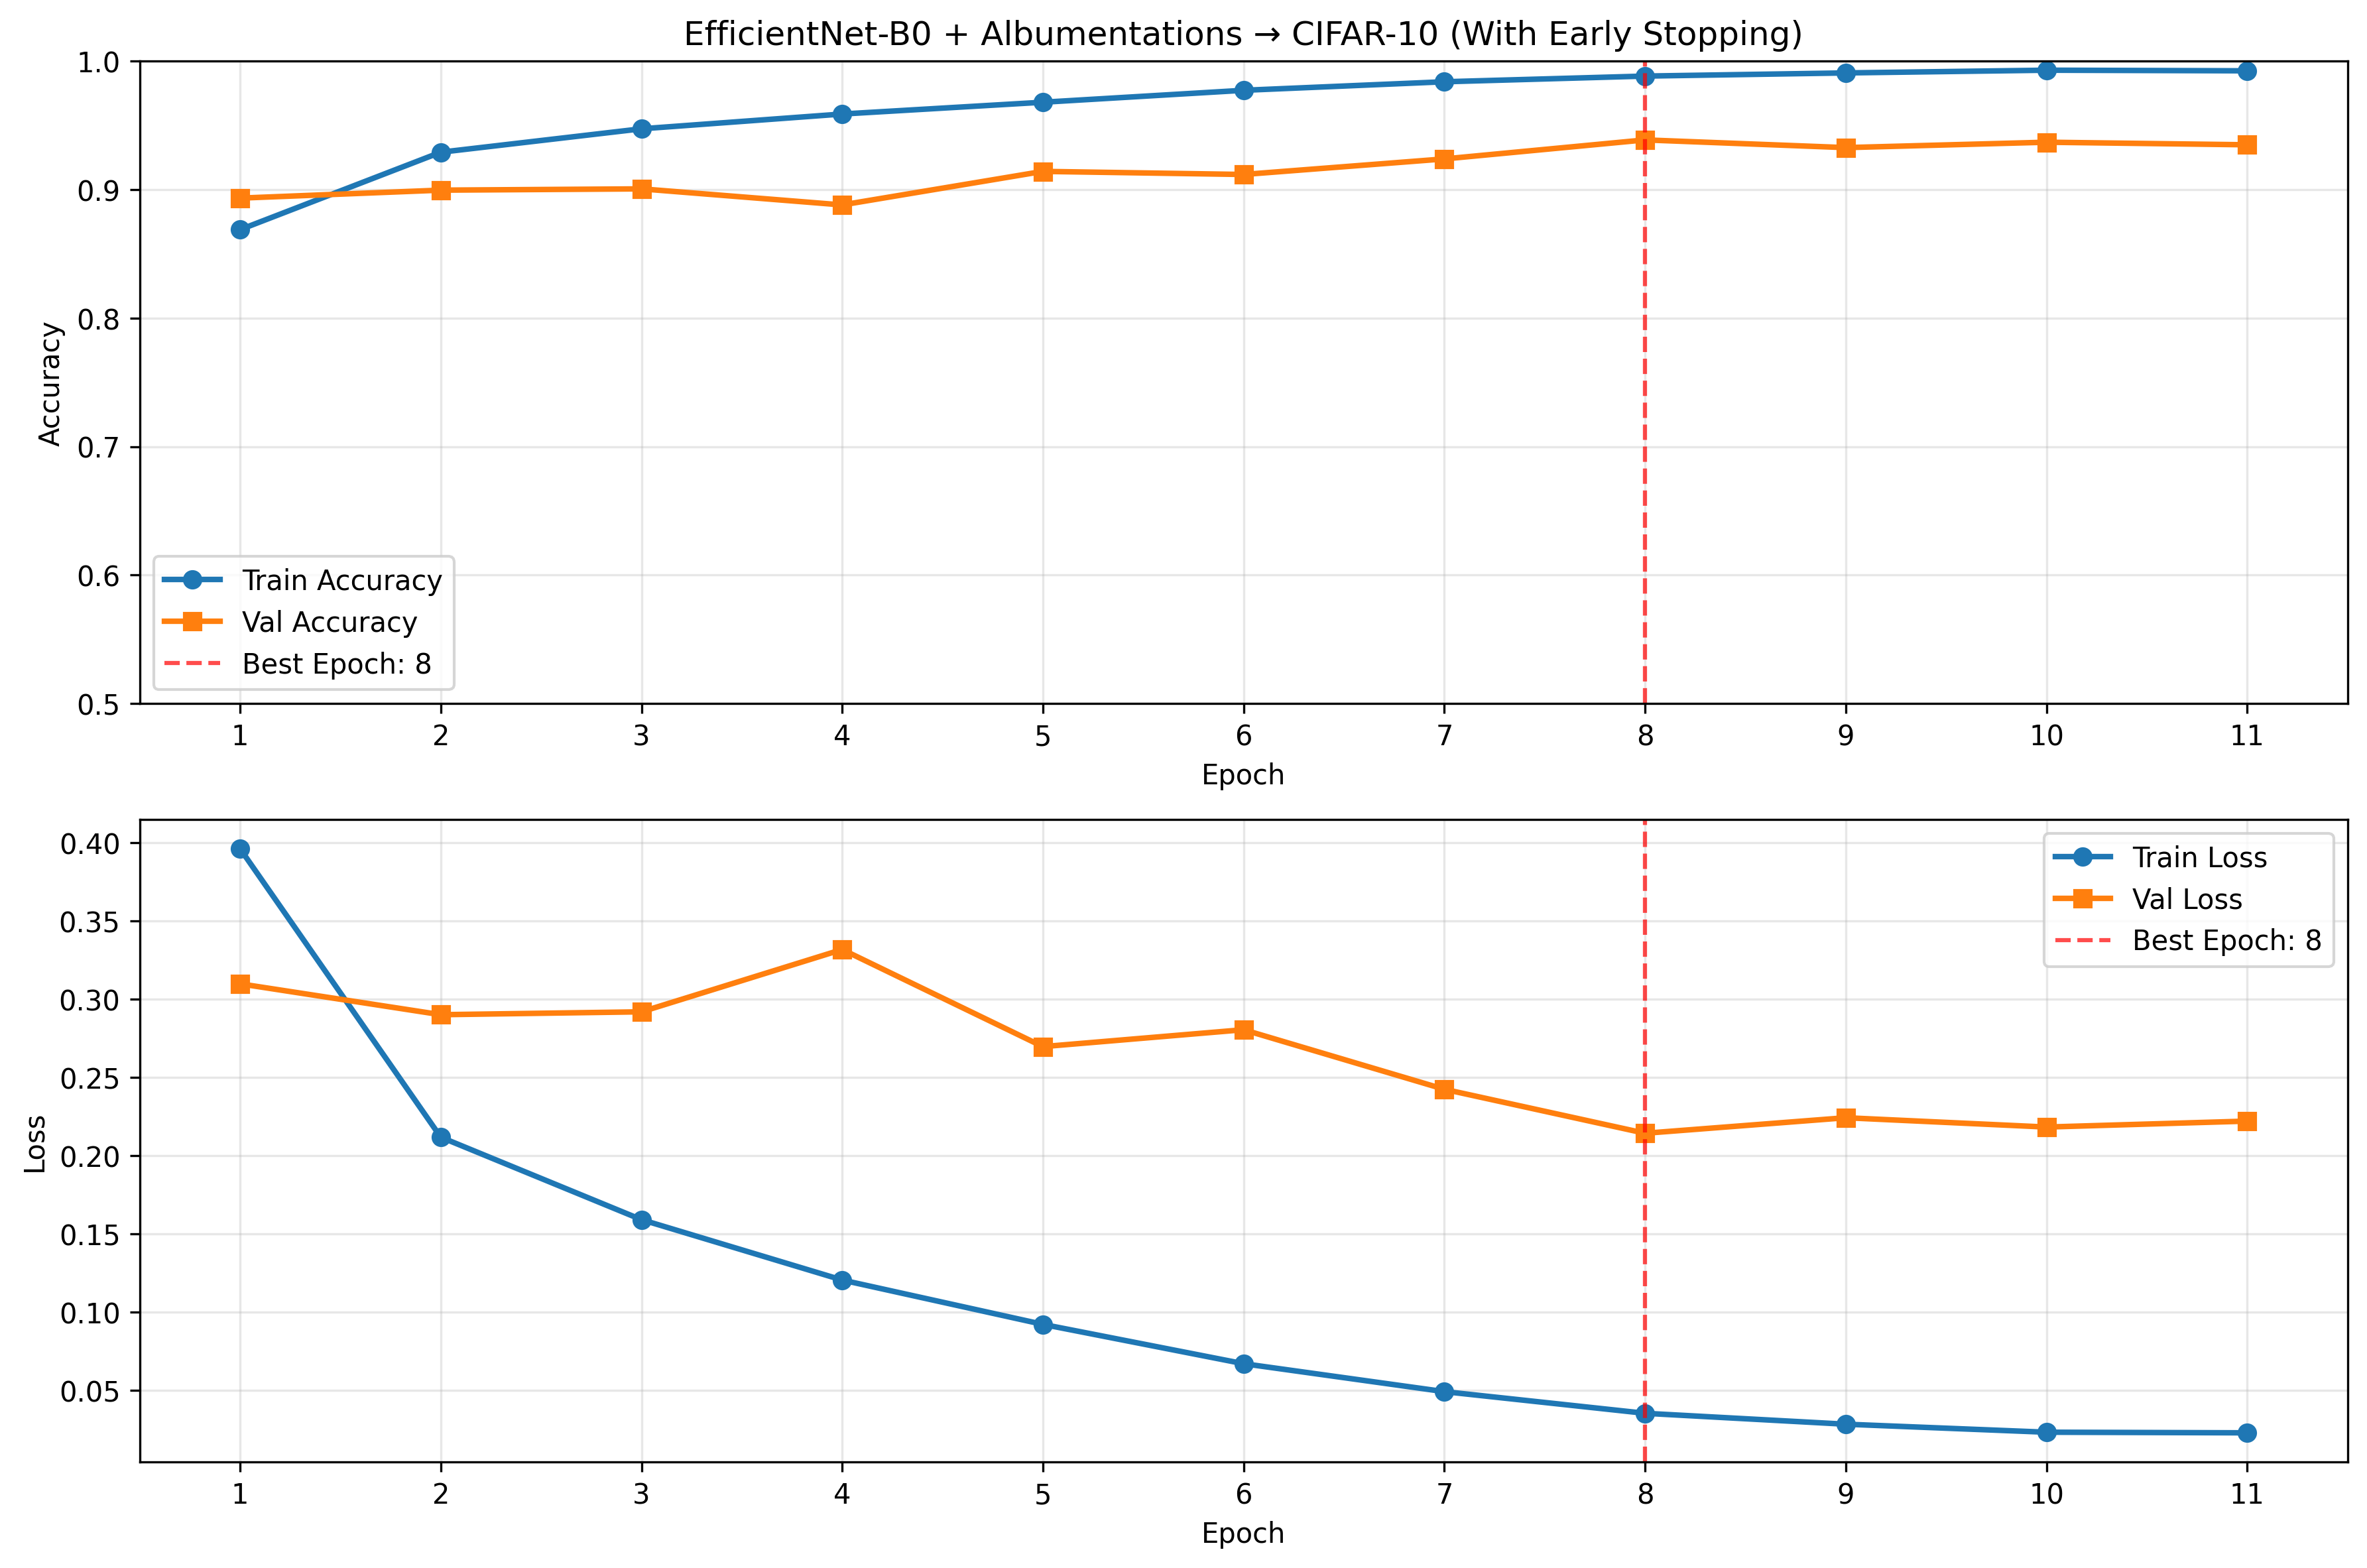
\includegraphics[width=0.8\textwidth]{docs/accuracy_plot_with_early_stopping.png}
    \caption{График точности дообученной EfficientNet-B0}
    \label{fig:accuracy_plot}
\end{figure}

\section{Latency}

Была измерена пропускная задержка при обработке отдельно взятого изображения (1000 прогонов). Результат представлен на рис. 3. После начального прогрева задержка колеблется в районе 8.79 для B3 и в районе 5.54 для B0.

\begin{figure}[ht]
    \centering
    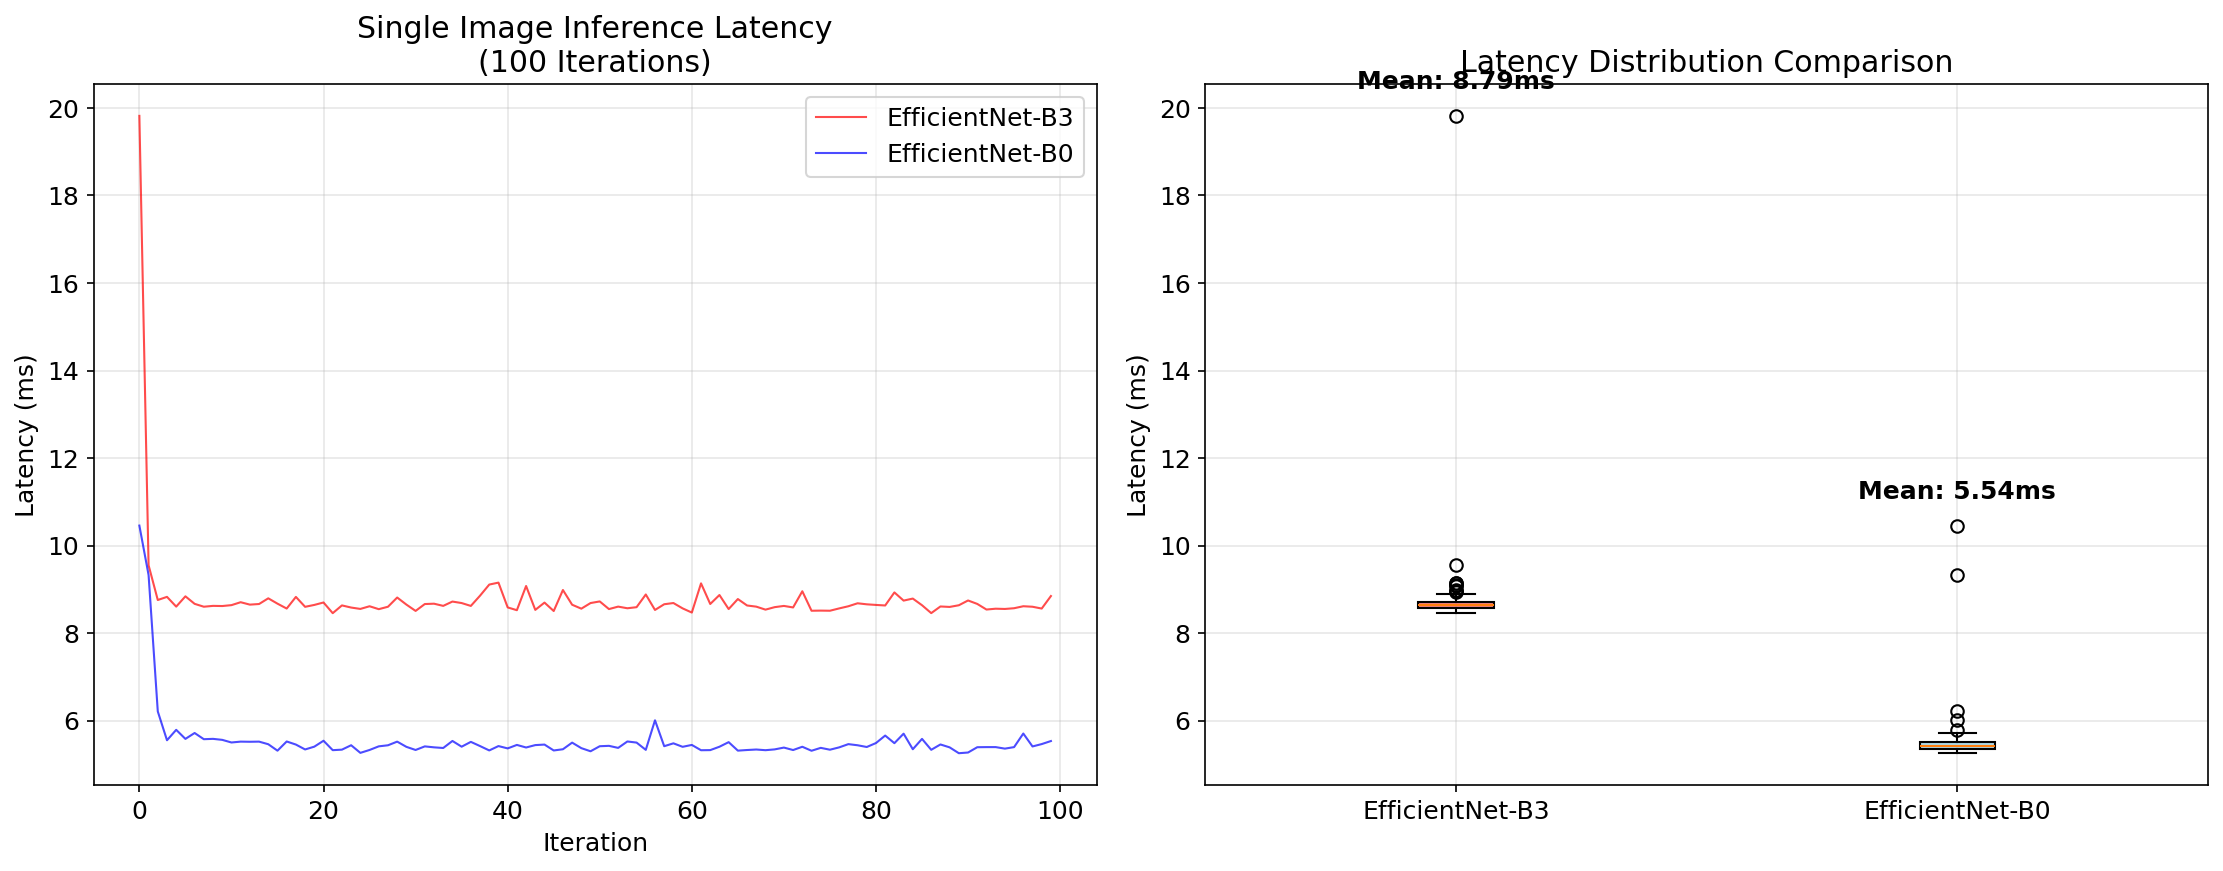
\includegraphics[width=1\textwidth]{docs/latency.png}
    \caption{График задержки на 1000 прогонах изображения}
    \label{fig:accuracy_plot}
\end{figure}

\section{TensorRT}

Попробовали использовать TensorRT в качестве бекенда. Непонятно зачем мы занялись такой глупостью на AMD. Результат ожидаемый.

\begin{figure}[ht]
    \centering
    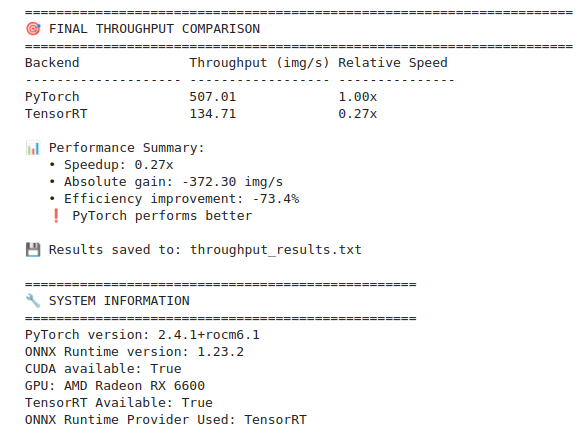
\includegraphics[width=0.8\textwidth]{docs/Screenshot from 2025-10-24 21-46-11.png}
    \caption{Выхлоп TensorRT vs. PyTorch}
    \label{fig:accuracy_plot}
\end{figure}

\section{Seaborn-barplot}

Сравнили скорость инференса PyTorch, ONNX и ONNX с квантизацией int8. Результат представлен на следующем изображении. 

\begin{figure}[ht]
    \centering
    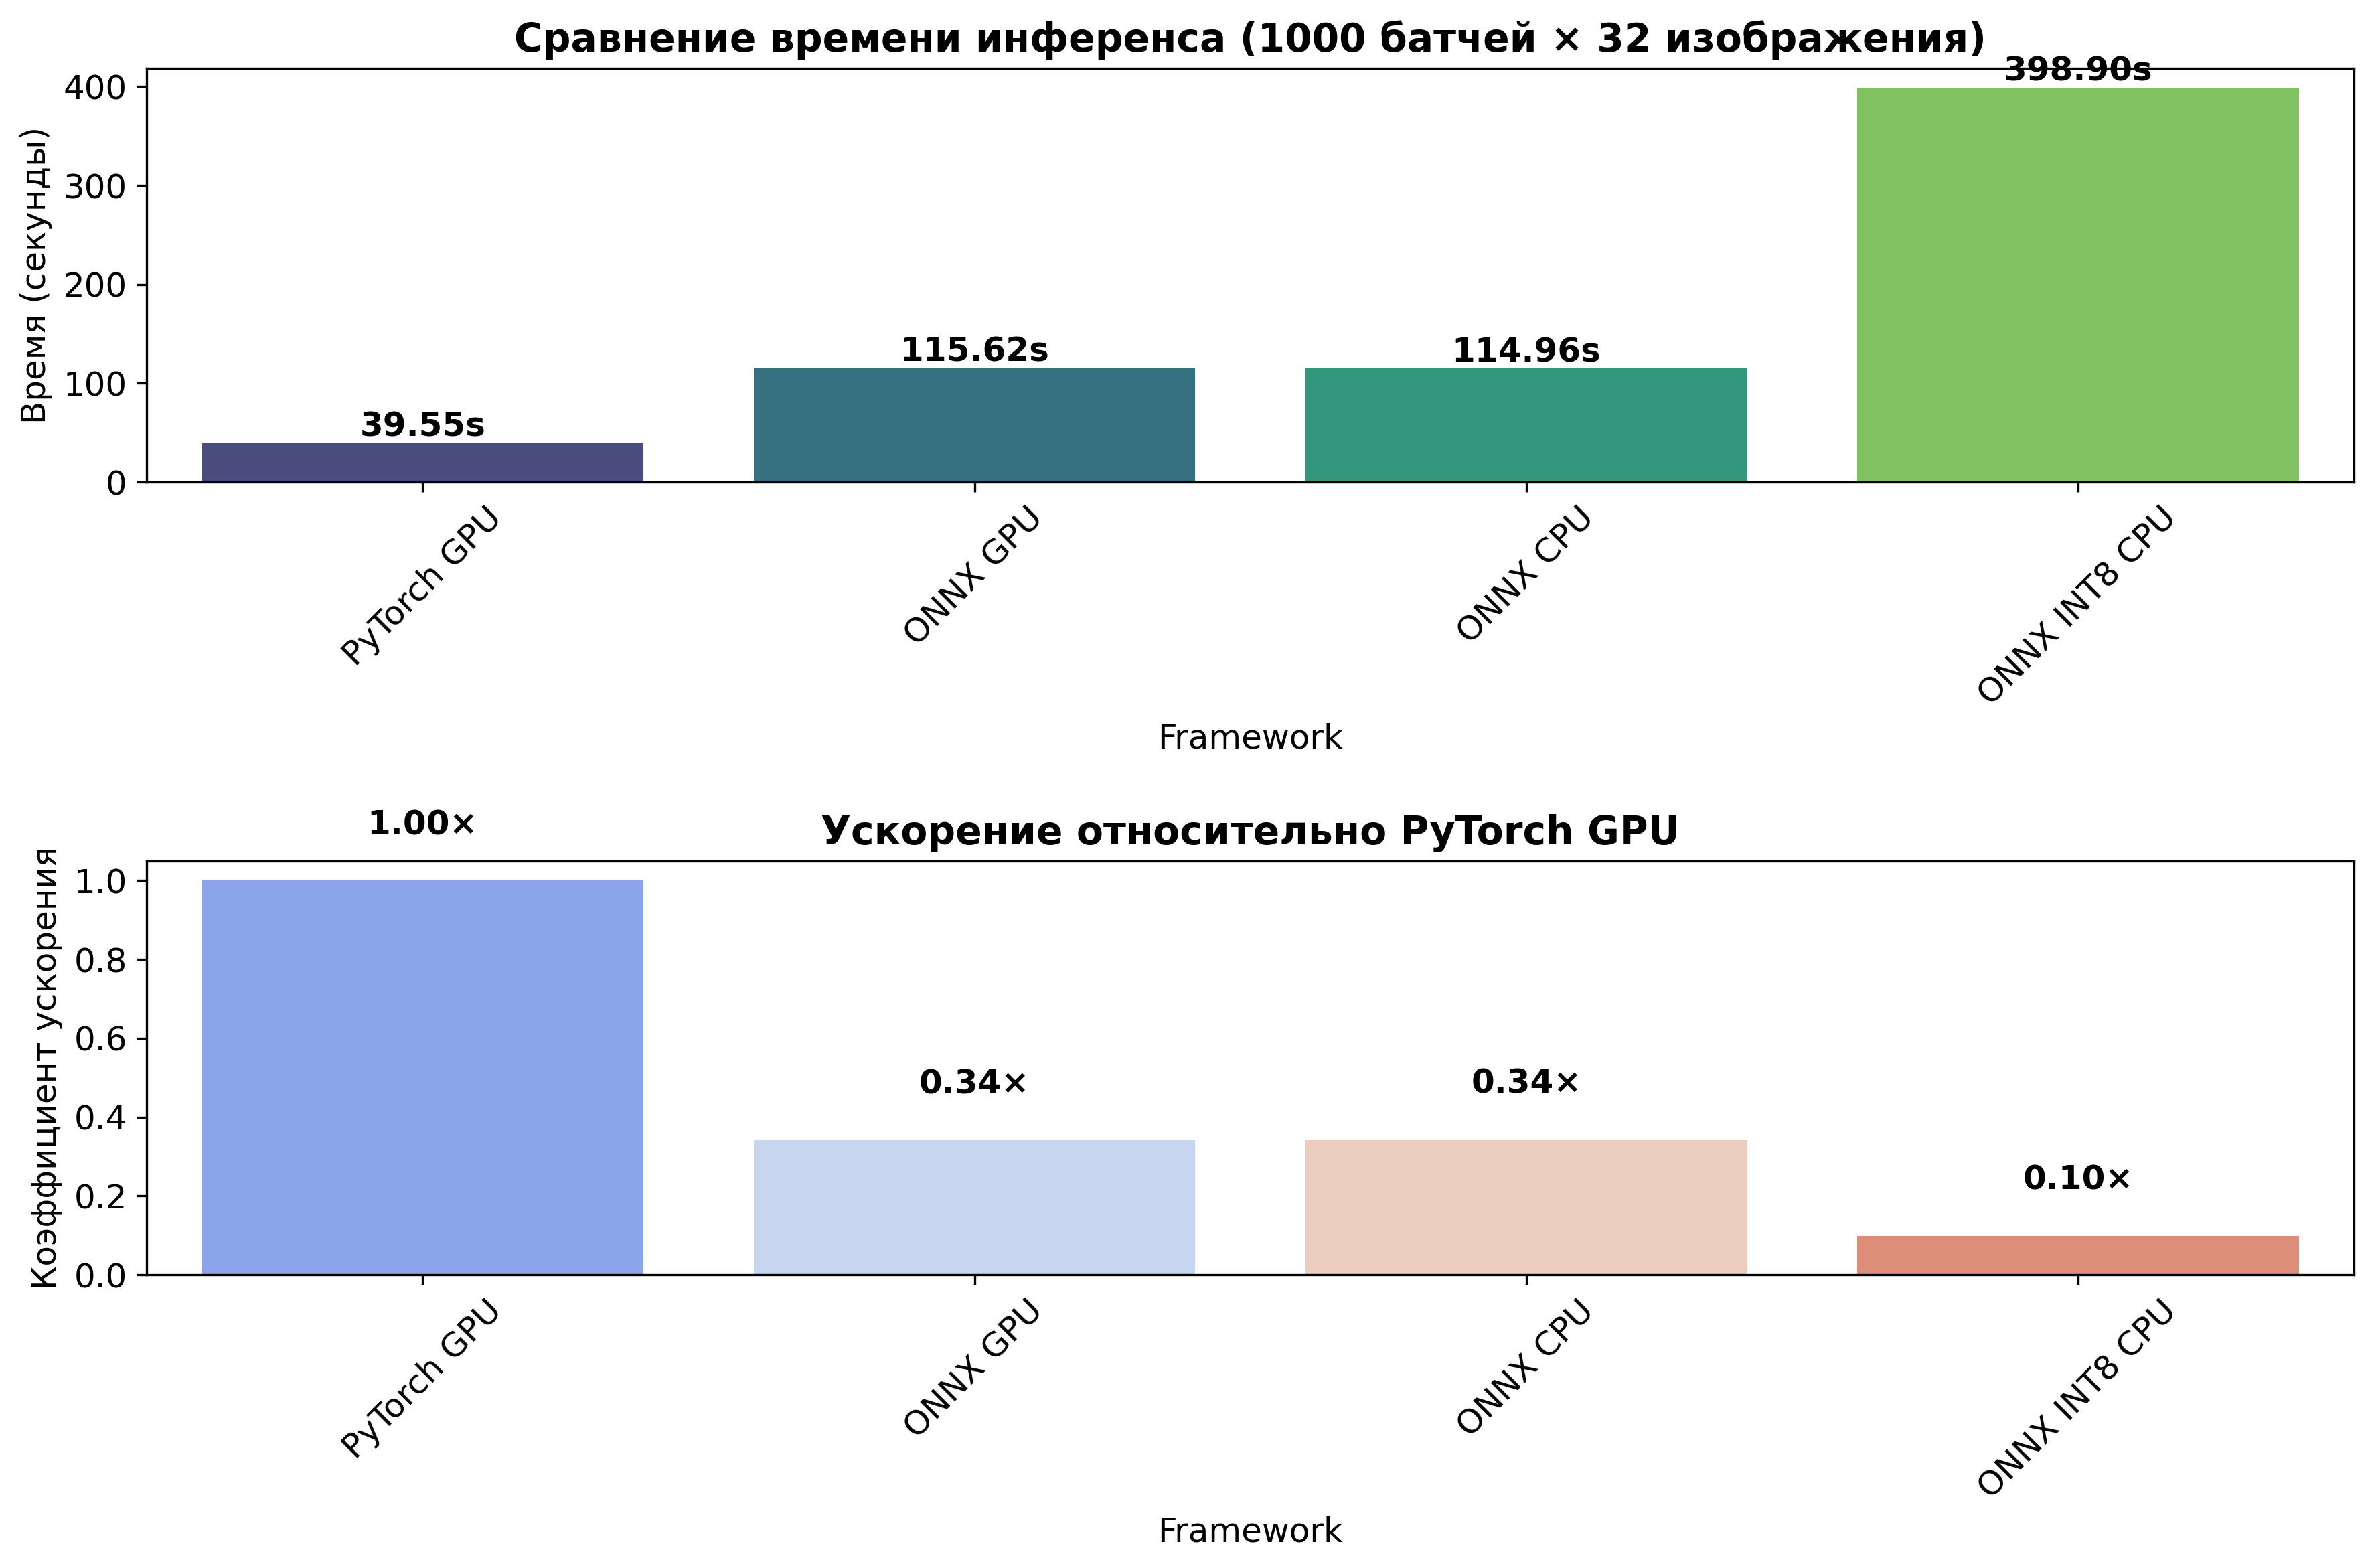
\includegraphics[width=1\textwidth]{docs/speedup.png}
    \caption{Графики PyTorch vs. ONNX vs. ONNX INT8}
    \label{fig:accuracy_plot}
\end{figure}

\section {INT8-точность}

Сравнили точность float32 и int8. Результат плачевный: int8 пытается везде увидеть автомобиль. Точность соответствующая.

\begin{figure}[ht]
    \centering
    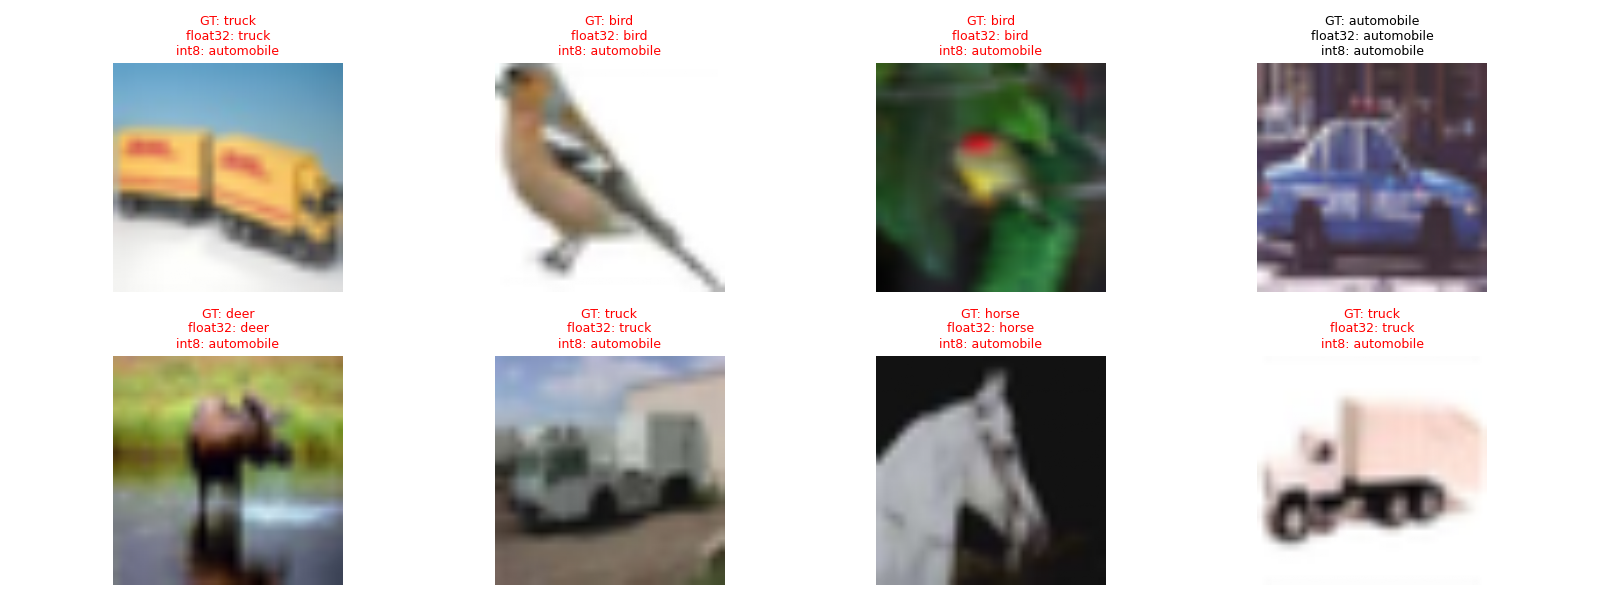
\includegraphics[width=1.2\textwidth]{docs/visualization.png}
    \caption{Сравнение квантов}
    \label{fig:accuracy_plot}
\end{figure}

\end{document}
